% Copyright 2004 by Till Tantau <tantau@users.sourceforge.net>.
%
% In principle, this file can be redistributed and/or modified under
% the terms of the GNU Public License, version 2.
%
% However, this file is supposed to be a template to be modified
% for your own needs. For this reason, if you use this file as a
% template and not specifically distribute it as part of a another
% package/program, I grant the extra permission to freely copy and
% modify this file as you see fit and even to delete this copyright
% notice. 

\documentclass{beamer}

% There are many different themes available for Beamer. A comprehensive
% list with examples is given here:
% http://deic.uab.es/~iblanes/beamer_gallery/index_by_theme.html
% You can uncomment the themes below if you would like to use a different
% one:
%\usetheme{AnnArbor}
%\usetheme{Antibes}
%\usetheme{Bergen}
%\usetheme{Berkeley}
%\usetheme{Berlin}
%\usetheme{Boadilla}
%\usetheme{boxes}
%\usetheme{CambridgeUS}
%\usetheme{Copenhagen}
%\usetheme{Darmstadt}
%\usetheme{default}
%\usetheme{Frankfurt}
%\usetheme{Goettingen}
%\usetheme{Hannover}
%\usetheme{Ilmenau}
%\usetheme{JuanLesPins}
%\usetheme{Luebeck}
\usetheme{Madrid}
%\usetheme{Malmoe}
%\usetheme{Marburg}
%\usetheme{Montpellier}
%\usetheme{PaloAlto}
%\usetheme{Pittsburgh}
%\usetheme{Rochester}
%\usetheme{Singapore}
%\usetheme{Szeged}
%\usetheme{Warsaw}

\usepackage{kotex}
\usepackage{braket}
\usepackage{array}
\usepackage{calc}
\usepackage{datetime}


\graphicspath{{images/}}
\usepackage{listings}

\newcommand\fig[2]{
\begin{figure}[h]
  \centering
  \includegraphics[width = \textwidth]{#1}
  \caption{#2} 
  \label{fig:#1}
\end{figure}
}

\usepackage{kotex} 
\usepackage{hyperref}
\usepackage{listings}
\usepackage{color}

\definecolor{dkgreen}{rgb}{0,0.6,0}
\definecolor{gray}{rgb}{0.5,0.5,0.5}
\definecolor{mauve}{rgb}{0.58,0,0.82}

\definecolor{mygreen}{rgb}{0,0.6,0}
\definecolor{mygray}{rgb}{0.5,0.5,0.5}
\definecolor{mymauve}{rgb}{0.58,0,0.82}

\lstset{ 
  backgroundcolor=\color{white},   % choose the background color; you must add \usepackage{color} or \usepackage{xcolor}; should come as last argument
  basicstyle=\footnotesize,        % the size of the fonts that are used for the code
  breakatwhitespace=false,         % sets if automatic breaks should only happen at whitespace
  breaklines=true,                 % sets automatic line breaking
  captionpos=b,                    % sets the caption-position to bottom
  commentstyle=\color{mygreen},    % comment style
  deletekeywords={...},            % if you want to delete keywords from the given language
  escapeinside={\%*}{*)},          % if you want to add LaTeX within your code
  extendedchars=true,              % lets you use non-ASCII characters; for 8-bits encodings only, does not work with UTF-8
  frame=single,	                   % adds a frame around the code
  keepspaces=true,                 % keeps spaces in text, useful for keeping indentation of code (possibly needs columns=flexible)
  keywordstyle=\color{blue},       % keyword style
  language=Python,                 % the language of the code
  morekeywords={*,...},            % if you want to add more keywords to the set
  numbers=left,                    % where to put the line-numbers; possible values are (none, left, right)
  numbersep=5pt,                   % how far the line-numbers are from the code
  numberstyle=\tiny\color{mygray}, % the style that is used for the line-numbers
  rulecolor=\color{black},         % if not set, the frame-color may be changed on line-breaks within not-black text (e.g. comments (green here))
  showspaces=false,                % show spaces everywhere adding particular underscores; it overrides 'showstringspaces'
  showstringspaces=false,          % underline spaces within strings only
  showtabs=false,                  % show tabs within strings adding particular underscores
  stepnumber=2,                    % the step between two line-numbers. If it's 1, each line will be numbered
  stringstyle=\color{mymauve},     % string literal style
  tabsize=2,	                   % sets default tabsize to 2 spaces
  title=\lstname                   % show the filename of files included with \lstinputlisting; also try caption instead of title
}


\lstdefinestyle{python}{frame=tb,
  language=Python,
  aboveskip=3mm,
  belowskip=3mm,
  showstringspaces=false,
  columns=flexible,
  basicstyle={\small\ttfamily},
  numbers=left,
  numberstyle=\tiny\color{gray},
  keywordstyle=\color{blue},
  commentstyle=\color{dkgreen},
  stringstyle=\color{mauve},
  breaklines=true,
  breakatwhitespace=true,
  tabsize=4
}


\title{Problems on Basic Data Structures}

% A subtitle is optional and this may be deleted
\subtitle{Koscom Algorithm Lecture}

\author{신승우}
% - Give the names in the same order as the appear in the paper.
% - Use the \inst{?} command only if the authors have different
%   affiliation.

% \institute[Universities of Somewhere and Elsewhere] % (optional, but mostly needed)
% {
  % \inst{1}%
  % Department of Computer Science\\
  % University of Somewhere
  % \and
  % \inst{2}%
  % Department of Theoretical Philosophy\\
  % University of Elsewhere}
% - Use the \inst command only if there are several affiliations.
% - Keep it simple, no one is interested in your street address.

% - Either use conference name or its abbreviation.
% - Not really informative to the audience, more for people (including
%   yourself) who are reading the slides online

\subject{Theoretical Computer Science}

% This is only inserted into the PDF information catalog. Can be left
% out. 

% If you have a file called "university-logo-filename.xxx", where xxx
% is a graphic format that can be processed by latex or pdflatex,
% resp., then you can add a logo as follows:

% \pgfdeclareimage[height=0.5cm]{university-logo}{university-logo-filename}
% \logo{\pgfuseimage{university-logo}}

% Delete this, if you do not want the table of contents to pop up at
% the beginning of each section:


% \AtBeginSection[]
% {
  % \begin{frame}[fragile]<beamer>{Outline}
    % \tableofcontents[currentsection,hideallsections]
  % \end{frame}
% }

% Let's get started
\begin{document}

\begin{frame}
  \titlepage
\end{frame}

\begin{frame}{Outline}
  \tableofcontents
  % You might wish to add the option [pausesections]
\end{frame}

% Section and sections will appear in the presentation overview
% and table of contents.

% \begin{frame}[fragile][fragile]{hello.py}
% 이제는 위에서 했던 것과 거의 비슷한 것을 할 텐데, 다만 다른 방식으로 해 볼 것입니다. 화면에서 보이는 대로 따라하세요. 
% \begin{lstlisting}[language=Python]
% print('Hello World!')
% \end{lstlisting}
% \end{frame}

\section{Directory Structure as Tree} 

% \begin{frame}{}

% \end{frame}

\section{Huffman Encoding/Decoding} 


% \begin{frame}{Huffman Encoding}

% \end{frame}


% \begin{frame}{}

% \end{frame}


\section{Expression Parsing}
\begin{frame}{What is Parsing?} 
\begin{block}{Parsing} 
특정 형식에 맞는 문자열을 원하는 데이터구조 형태로 만드는 것
\end{block}
\begin{itemize} 
\item \textbf{특정 형식}에 맞는 문자열 : Formal Grammar 
\item \textbf{원하는 데이터구조} : Abstract Syntax Tree(AST)
\end{itemize}
\end{frame}

% use for later slides on special lectures 
% \begin{frame}{Formal Grammar} 
% \begin{block}{Formal Grammar} 
% 형식 문법은 $N, T, P, S$의 4-tuple을 뜻하며, 각각은 다음과 같다.
% \end{block}
% \begin{itemize}
% \item N : Nonterminal Symbol 
% \item T : Terminal Symbol 
% \item P : production rules 
% \item S : Starting Symbol 
% \end{itemize}
% \end{frame}


% \begin{frame}{Formal Grammar} 
 
% 이 때, 각각은 다음의 조건을 만족해야 한다. 
% \begin{itemize}
% \item $N \cup T = \phi$
% \item $S \in N$
% \item P의 원소들은 $(N \cup T)*N(N \cup T)* -> (N \cup T)*$ 의 꼴. 
% \end{itemize}
% \end{frame}




\begin{frame}{수식의 Grammar} 
수식의 grammar를 살펴보면 다음과 같다. \\
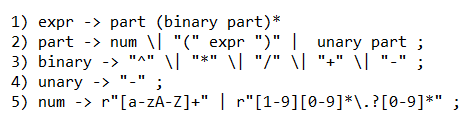
\includegraphics[width=10cm,keepaspectratio]{grammar}

1)에서 (binary part)*는 binary part의 유한한 반복을 뜻한다. 0번 반복하더라도 상관없다. 

\end{frame}

\begin{frame}{Syntax Check using Grammar}
위 문법에 기반하여 $x*(y+z)$ 가 수식의 문법에 맞는 문장인지 알아보자. 

\begin{table}[]
\centering
\caption{$x*(y+z)$ 체크}
\label{my-label}
\begin{tabular}{|l|l|l|}
\hline
current string & rule & result \\ \hline
x*(y+z)&1    & is x part?, is * binary?, is (y+z) part?      \\ \hline
x &  2, 3 & x is num! / num is part!      \\ \hline
*& 3    & * is binary!      \\ \hline
(y+z)& 3    &  is y+z expr?      \\ \hline
y, z& same to x    &   y,z is num! / num is part!   \\ \hline
+ & 3    &  + is binary!     \\ \hline
\end{tabular}
\end{table}

\end{frame}

\begin{frame}{Syntax Check using Grammar} 
이번에는 $x*(y+$ 가 수식의 문법에 맞는 문장인지 알아보자. 

\begin{table}[]
\centering
\caption{$x*(y+$ 체크}
\label{my-label}
\begin{tabular}{|l|l|l|}
\hline
current string & rule & result \\ \hline
x*(y+ & 1    & is x part?, is * binary?, is (y+ part?      \\ \hline
x &  2, 3 & x is num! / num is part!      \\ \hline
*& 3    & * is binary!      \\ \hline
(y+& 3    &  is y+ expr?      \\ \hline
y & same to x    &   y is num! / num is part!   \\ \hline
+ & 3    &  + is binary!     \\ \hline
eos &  None  &  expected part, return eos : \textbf{SyntaxError}     \\ \hline
\end{tabular}
\end{table}
이처럼, 위 문법에서의 규칙들을 순차적으로 적용하는 것으로 특정 문자열이 그 문법에 맞게 작성되었는지를 알 수 있다. 이럴 때 그 특정 문자열은 그 문법에 의해서 생성되었다고 한다. 

\end{frame}


\subsection{Abstract Syntax Tree} 

\begin{frame}{Abstract Syntax Tree} 

구문의 문법 구조를 반영하여 트리 형태로 나타낸 것을 abstract syntax tree라고 한다. 예를 들어서, 위 $x*(y+z)$의 경우 다음과 같은 트리로 생각할 수 있다. 

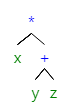
\includegraphics[height=5cm,keepaspectratio]{ast}

이때까지 문법과 그 문법을 이용하여 파싱한 결과물이 무엇인지 간략하게 살펴보았다. 이제 본격적으로 어떤 식으로 구현하는지 살펴 보고자 한다. 

\end{frame}


\subsection{Recursive Descent Algorithm}

\begin{frame}{Parser Structure} 

먼저, 일반적인 파서의 구조를 살펴보자. 일반적으로 파서는 두 가지 함수로 이루어져 있다. 

\begin{itemize} 
\item tokenizer : string to tokens
\item parser : tokens to AST
\end{itemize}

여기서, token이란 최소한의 의미를 가지는 문자열을 말한다. 문법에서 "으로 둘러싸인 문자열이나 그 문자열이 나타내는 정규표현식과 일치하는 문자열을 뜻한다. 

\end{frame}

\begin{frame}{Implementing Tokenizer} 

Tokenizer의 경우, 다음의 과정을 통해서 만들 수 있다. 

\begin{itemize} 
\item 문법에서 token의 패턴을 추출한다. 
\item input string에 대해서, input string == '''' 가 될 때까지 
\begin{itemize}
\item 각 패턴에 대해서 check re.match(pattern, input string)
\item 만약 맞으면 input string에서 pattern과 일치하는 부분을 yield
\item 일치하는 부분을 제외한 나머지를 input string으로 업데이트
\item 만약 모든 패턴에 대해서 맞지 않으면 SyntaxError 리턴
\end{itemize}
\end{itemize}
\end{frame}

\begin{frame}{Shunting-Yard Algorithm} 

이제 얻어진 token들을 이용하여 abstract syntax tree를 만드는 알고리즘을 생각해 보자. 먼저, 스택 2개를 생각한다. 

\begin{itemize} 
\item operand stack 
\item operation stack 
\end{itemize}

이 때, operation stack에서는 필요한 operand들이 파싱이 끝날 때까지 operation을 pop하지 않는다. 또한, operation들 중 더 우선순위가 높은 operation이 항상 스택의 위에 오도록 유지한다. 예를 들어서, operation stack에 /가 있을 때, +가 들어오기 전에 /를 pop하고 필요한 처치를 한다. 즉, 그 때 operand stack의 가장 위에 있는 token 2개를 pop\footnote{만약 operation이 unary라면 1개. operation에 맞는 갯수를 리턴하면 된다.}  하여 Tree('/', tok1, tok2) 형태로 만드는 것이다. 만약 그 때 operand stack에 2개의 token이 없다면 에러를 리턴한다. operator가 스택에서 pop될 때마다 tree가 하나씩 생성되며, 이를 다시 operand stack에 push한다.

파싱이 되는 예시 2개와, 되지 않는 예시 1개를 들어서 살펴보고 이를 구현해보겠다. 

\end{frame}

\begin{frame}{예시}
\begin{table}[]
\centering
\caption{$x*y+z$ 파싱 예제}
\label{my-label}
\begin{tabular}{|l|l|l|l|}
\hline
tokens & operand  & op  & action \\ \hline
x, *, y, +, z &     &  & operand.push(x)     \\ \hline
*, y, +, z &  x   &  & compare(*, None)     \\ \hline
, y, +, z &  x   & * & operation.push(*)    \\ \hline
y, +, z &  x   & * & operand.push(y)     \\ \hline
+, z &  y, x  & * & compare(*, +)     \\ \hline
+, z &  Tree(*, [x, y])   &  & operator.pop()     \\ \hline
z &  Tree(*, [x, y])   & + & operation.push(+)     \\ \hline
&  z, Tree(*, [x, y])   & + & operand.push(z)     \\ \hline
&  Tree(+, [z, Tree(*, [x, y])])   &  & operation.pop()     \\ \hline
\end{tabular}
\end{table}


\end{frame}



\begin{frame}{예시}

\begin{table}[]
\centering
\caption{$x*(y+z)$ 파싱 예제}
\label{my-label}
\begin{tabular}{|l|l|l|l|}
\hline
tokens & operand  & op  & action \\ \hline
x, *, (,  y, +, z, )&     &  & operand.push(x)     \\ \hline
*, (,  y, +, z, )&  x  &  & operation.push(*)     \\ \hline
(,  y, +, z, )&  x  & * & parse(find\_match(tokens, 0))     \\ \hline
 &  Tree(+, [y,z]) x  & * & operand.push(parse(..))     \\ \hline
 &  Tree(+, [y,z]) x  & * & operator.pop()     \\ \hline
 &  Tree(*, [Tree(+, [y,z]), x])  &  & operator.pop()     \\ \hline
\end{tabular}
\end{table}

여기서 find\_match 함수를 사용하는데, 이는 tokens에서 어떤 index의 괄호와 쌍을 이루는 괄호를 찾는 것이다. 이를 통해서 괄호 안의 식을 우선적으로 처리할 수 있다. 

\end{frame}


\begin{frame}{예시}

\begin{table}[]
\centering
\caption{$y+$ 파싱 예제}
\label{my-label}
\begin{tabular}{|l|l|l|l|}
\hline
tokens & operand  & op  & action \\ \hline
y, + &     &  & operand.push(y)     \\ \hline
 + &  y   &  & operator.push(+)     \\ \hline
 &  y   & + & operator.pop()     \\ \hline
 &  y   & + & operand.pop();operand.pop()     \\ \hline
 &  y   & + & raise SyntaxError     \\ \hline
\end{tabular}
\end{table}

\end{frame}


\begin{frame}{Implementing Parser} 

위에서 알고리즘의 개요를 살펴보았다. 이제 본 알고리즘을 구현해볼 것이다. 본격적인 구현 전에, 필요한 변수들과 함수들을 구현하자. 
\begin{itemize} 
\item precedence : operator들 간 우선순위를 저장한 변수
\item find\_match 함수 : 맞는 괄호 찾아주기 
\item compare 함수 : operator 간 우선순위 비교
\end{itemize}

이후, 스택 두 개를 만들어 위 알고리즘을 구현한다. 
\end{frame}

\begin{frame}{Implementing Parser : 실습}
 
파싱하고자 하는 expression의 문법은 다음과 같습니다. 

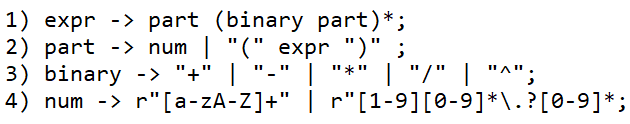
\includegraphics[width=10cm,keepaspectratio]{simplegrammar}

실습에서는 
\begin{itemize} 
\item operator 순서는 \textasciicircum, (*, /), (+, -) 순입니다. 
\item \textbf{unary는 고려하지 않습니다.}
\item parser은 문법에 맞게 syntax tree형태로 식을 파싱하여 반환하면 됩니다. 
\end{itemize} 


\end{frame}


\end{document}


